\subsection{The Disordered Ising Model}
\label{ssec:isingmodel}
    The examined model is a modified 2D Ising model.
    The most common definition of the Ising model, to which will be referred
    as the \emph{standard Ising model}, is a square lattice with edge length \(L\) and
    \(N=L^2\) sites. Each site has a magnetic moment, the spin. Each
    spin can take a value \(s \in \{-1,+1\}\) and interacts with its
    nearest neighbors described by the Hamiltonian from eq. \eqref{eq:hamiltonian}
    \begin{equation}
        H = - \sum_{\avg{i,j}}J_{ij}s_{i}s_{j} - \sum_i \tilde{H}_i s_i
        \label{eq:hamiltonian}
    \end{equation}
    \(\avg{i,j}\) refers to nodes \(i\) and \(j\) which are nearest
    neighbors. And \(J_{ij}\) is the coupling constant between \(i\) and
    \(j\). If \(J_{ij} > 0 \ \forall i,j\) the model resembles a ferromagnet.
    \(\tilde{H}_i\) denotes the outer magnetic field at the position of
    site \(i\).\\
    In this thesis \(\tilde{H}_i=0 \ \forall i\). The most important
    modification is, that the sites of the square lattice are displaced.
    The displacement is randomly Gauß distributed with the standard
    deviation \(\sigma\), i.e.\ the \(x\) and \(y\) coordinates of the
    sites are displaced by random \(\Delta x\) and \(\Delta y\) drawn
    from a Gauß distribution eq. \eqref{eq:gauss}.
    This is sketched in fig. \ref{fig:displacement}.
    \begin{equation}
        f(x)=\frac{1}{\sqrt{2\pi}\sigma}\mathrm{e}^{-\frac{x^2}{2\sigma^2}}
        \label{eq:gauss}
    \end{equation}
    \[x \to x + \Delta x\]
    \[y \to y + \Delta y\]
    \begin{figure}[htbp]
        \centering
        \begin{tikzpicture}[scale=1.5, declare function={
        normal(\x,\m,\y) = 1/exp((\x-\m)*(\x-\m)/2/(\s^2))-\y;
      }]
    \def\s{0.5}

    \draw[dashed] (-2,0) -- (4,0);
    \draw[dashed] (0,-2) -- (0,2);
    \draw[dashed] (2,-2) -- (2,2);

    \def\dxa{0.4}
    \def\dya{-0.8}

    \draw (\dxa,\dya) -- node [below] {$\Delta x$} (0,\dya);
    \draw (\dxa,\dya) -- node [right] {$\Delta y$} (\dxa,0);
    \draw[loosely dotted] (\dxa,0) -- (\dxa,{1.6+normal(\dxa,0,0)});
    \draw[loosely dotted] (0,\dya) -- ({-1.6-normal(\dya,0,0)},\dya);
    \draw[->] (0,0) -- (0+\dxa*0.9,0+\dya*0.9);

    \draw[color=black,domain=-1.5:1.5] plot [smooth] (\x,{normal(\x,0,0)+1.6}) node[right] {};
    \fill (0, 0) circle(0.08);
    \draw[color=black] (0+\dxa, 0+\dya) circle(0.08);
    \draw[color=black,domain=-1.5:1.5,rotate=90] plot [smooth] (\x,{normal(\x,0,0)+1.6}) node[right] {};

    \draw[|-|] (-\s,2.8) -- node [above] {$\sigma$} (\s,2.8);
    \draw[|-|] (-2.8,-\s) -- node [left] {$\sigma$} (-2.8,\s);


    \def\dxb{0.5}
    \def\dyb{0.2}

    \draw[color=gray] (2+\dxb,0+\dyb) -- node [above] {$\Delta x_{2}$} (2, \dyb);
    \draw[color=gray] (2+\dxb,0+\dyb) -- node [right] {$\Delta y_{2}$} (2+\dxb,0);
    \fill[color=gray] (2, 0) circle(0.08);
    \draw[color=gray] (2+\dxb, 0+\dyb) circle(0.08);
\end{tikzpicture}

        \caption[Sketch how the Displacement Works]
        {
            Sketch how the displacement of the nodes works. The nodes
            get displaced by \(\Delta x\) and \(\Delta y\) drawn from the
            distributions displayed next to the points. The original
            square lattice is indicated by dashed lines.
        }
        \label{fig:displacement}
    \end{figure}\\
    This \(\sigma\) is also called \emph{disorder parameter} in the following.
    Because most sites will only have one nearest neighbor after the
    displacement, the lattice would collapse to many very small clusters.
    To avoid this, the new "nearest" neighbors are those sites connected
    by an edge. The edges are constructed according to
    one of the two in section \ref{ssec:graphtypes} defined rules,
    so that the lattice represents a proximity graph. Note that edges
    of a proximity graph do not cross each other, hence the 2D character
    of the lattice is preserved. The coupling constant \(J\) gets
    identified with edge weights. The weight of an edge \(E_{ij}\) is
    \(J_{ij} = \exp (\alpha (1-d_{ij}))\) where \(d_{ij}\) is the Euclidean
    distance between the nodes \(i\) and \(j\). The free parameter
    \(\alpha\) is set to \(\alpha = 0.5\) inspired by \cite{Lima2000}.
    The boundary is periodic e.g.\ nodes near the right edge can be
    connected to nodes near the left edge and vice versa. Analogous the
    top and bottom edges are connected. One can imagine that the model
    lives on the surface of a torus as pictured in fig. \ref{fig:torusRNG}.
    In subsequent graphics, the graphs will be unwrapped to rectangular
    shapes. Connections which cross a periodic boundary are indicated
    by edges which connect to an dashed node.
    \begin{figure}[htbp]
        \centering
        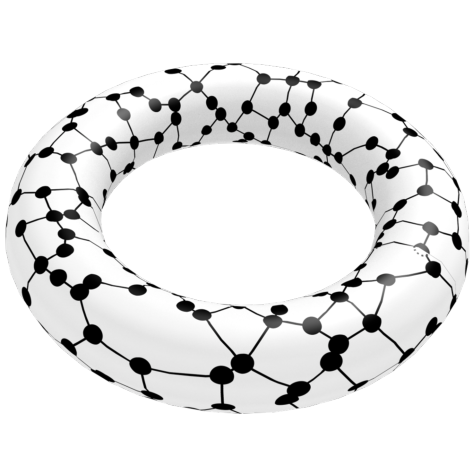
\includegraphics[width=0.45\textwidth]{images/torus}
        \caption[A Graph on a Torus to Visualise Periodic Boundary Conditions]
        {
            A graph on a torus to visualize periodic boundary conditions.
            Note that the lattice on this torus is not a square but has
            a height to width ratio of 1:4. At 1:1 the torus would cut
            itself. Hence, the torus represents the geometry of the model
            not perfectly, but gives very quick the right idea.
            %Also the shades are of course only a guide to the eye.
        }
        \label{fig:torusRNG}
    \end{figure}\\
    For \(\sigma = 0\) this is the standard Ising model with \(J = 1\),
    for which exists an analytic solution \cite{Onsager1944}. And for
    \(\sigma \gtrsim 1\) the nodes are distributed randomly. This case
    is already studied for constant \(J\) on the Delaunay triangulation
    in \cite{Janke1994}.\\

\subsection{Gabriel- and Relative Neighborhood Graph}
\label{ssec:graphtypes}
    A graph \(G(V,E)\) is a set of nodes \(V\) and edges \(E\).\\
    All here mentioned graph types are \emph{proximity graphs}. They are
    connecting nodes which are by some metric near to each other.
    Hence they are suited to generalize problems defined on regular
    lattices with nearest neighbor relationships, like the Ising model
    from the section \ref{ssec:isingmodel}.
    In this thesis the distance is always determined by the Euclidean
    metric in two dimensions, though in principle every metric in any
    dimension can be used.\\

    The Gabriel graph (GG) \cite{Gabriel1969} is a subgraph of the
    Delaunay triangulation. Two nodes \(i\) and \(j\) with distance
    \(d_{ij}\) are connected with an edge, if a circle with its
    center on half way between \(i\) and \(j\) and radius
    \(r = \frac d 2\) contains no other nodes. This area will be
    called \emph{lune} in the following. See also Figure
    \ref{fig:lunes}\subref{sfig:lunes:def}.\\
    The Relative Neighborhood graph (RNG) \cite{Toussaint1980} is a
    subgraph of the GG. Two nodes \(i\) and \(j\) with
    distance \(d_{ij}\) are connected, if no other node is in the
    \emph{lune}. The lune is defined as the intersection of two
    circles with radius \(r = d\) and centers on \(i\) and \(j\).
    See also Figure \ref{fig:lunes}\subref{sfig:lunes:def}.
    \begin{figure}[htbp]
        \centering
        \subfigure[Definition of the Lunes][]{
            \label{sfig:lunes:def}
            \tikzset{
    hatch distance/.store in=\hatchdistance,
    hatch distance=10pt,
    hatch thickness/.store in=\hatchthickness,
    hatch thickness=2pt
}

\makeatletter
\pgfdeclarepatternformonly[\hatchdistance,\hatchthickness]{flexible hatch no}
{\pgfqpoint{0pt}{0pt}}
{\pgfqpoint{\hatchdistance}{\hatchdistance}}
{\pgfpoint{\hatchdistance-1pt}{\hatchdistance-1pt}}%
{
    \pgfsetcolor{\tikz@pattern@color}
    \pgfsetlinewidth{\hatchthickness}
    \pgfpathmoveto{\pgfqpoint{0pt}{0pt}}
    \pgfpathlineto{\pgfqpoint{\hatchdistance}{\hatchdistance}}
    \pgfusepath{stroke}
}
\makeatletter
\pgfdeclarepatternformonly[\hatchdistance,\hatchthickness]{flexible hatch nw}
{\pgfqpoint{0pt}{0pt}}
{\pgfqpoint{\hatchdistance}{\hatchdistance}}
{\pgfpoint{\hatchdistance-1pt}{\hatchdistance-1pt}}%
{
    \pgfsetcolor{\tikz@pattern@color}
    \pgfsetlinewidth{\hatchthickness}
    \pgfpathmoveto{\pgfqpoint{0pt}{\hatchdistance}}
    \pgfpathlineto{\pgfqpoint{\hatchdistance}{0pt}}
    \pgfusepath{stroke}
}

\begin{tikzpicture}
    \clip (-2,2.25) rectangle (2,-1.75);

    \begin{scope}
        \clip (-1, 0.5) circle(2.06155281281);
        %~ \fill[fill=blue!20] (1, 0) circle(2.06155281281);
        %~ \draw[pattern=north west lines] (1, 0) circle(2.06155281281);
        \draw[pattern=flexible hatch no,hatch distance=10pt,hatch thickness=0.7pt] (1, 0) circle(2.06155281281);
    \end{scope}

    %~ \fill[fill=white] (0, 0.25) circle(1.0307764064);
    %~ \draw[pattern=north east lines] (0, 0.25) circle(1.0307764064);
    \draw[pattern=flexible hatch nw,hatch distance=10pt,hatch thickness=0.7pt] (0, 0.25) circle(1.0307764064);
    \draw[thick] (0, 0.25) circle(1.0307764064);

    \draw[thick] (-1, 0.5) circle(2.06155281281);
    \fill (-1, 0.5) circle(0.1);
    \draw[thick] (1, 0) circle(2.06155281281);
    \fill (1, 0) circle(0.1);
    \draw[thick] (1, 0) -- (-1, 0.5);
\end{tikzpicture}

        }
        \subfigure[RNG example][]{
            \label{sfig:lunes:rng}
            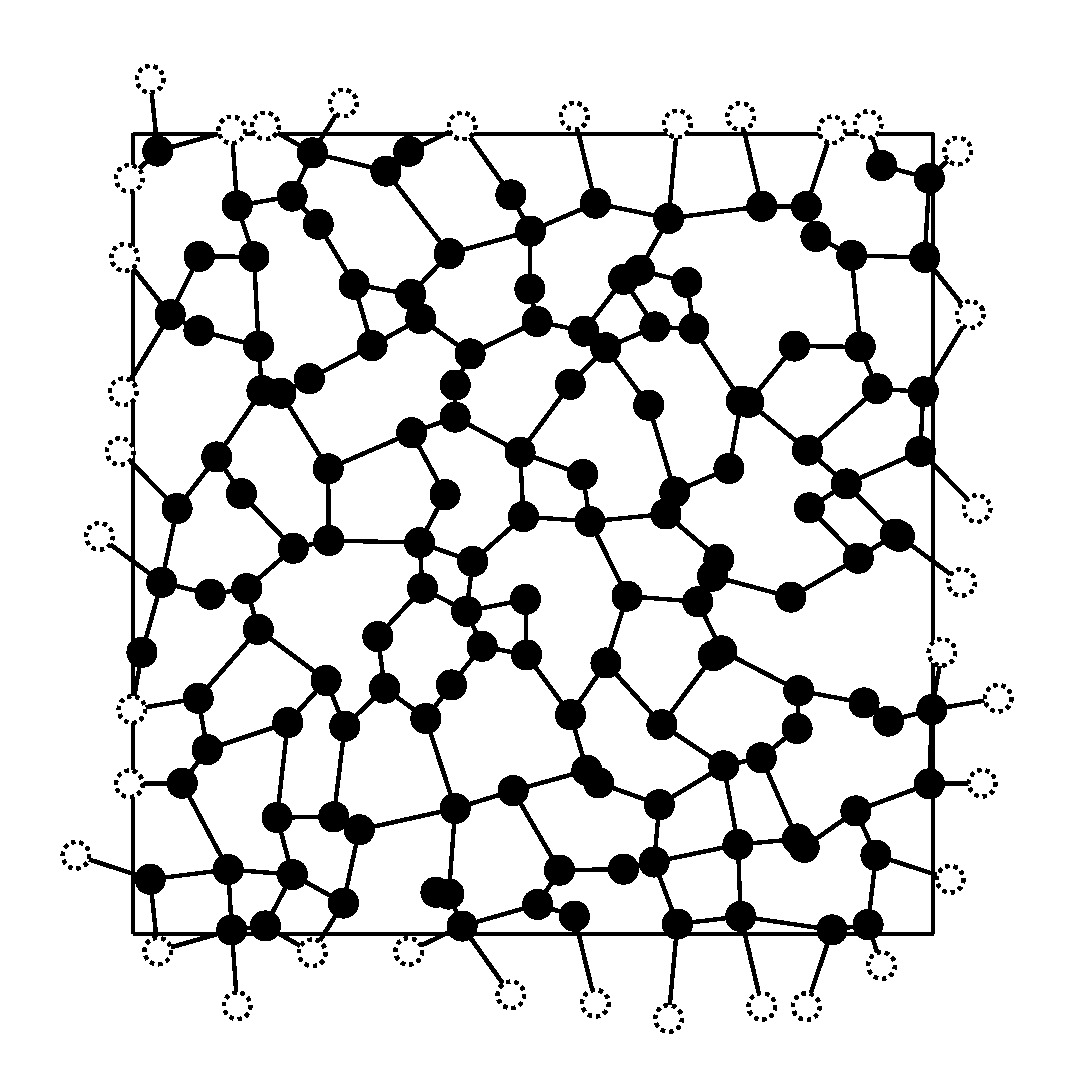
\includegraphics[width=0.3\textwidth]{images/RNG/L12S03.pdf}
        }
        \subfigure[GG example][]{
            \label{sfig:lunes:gg}
            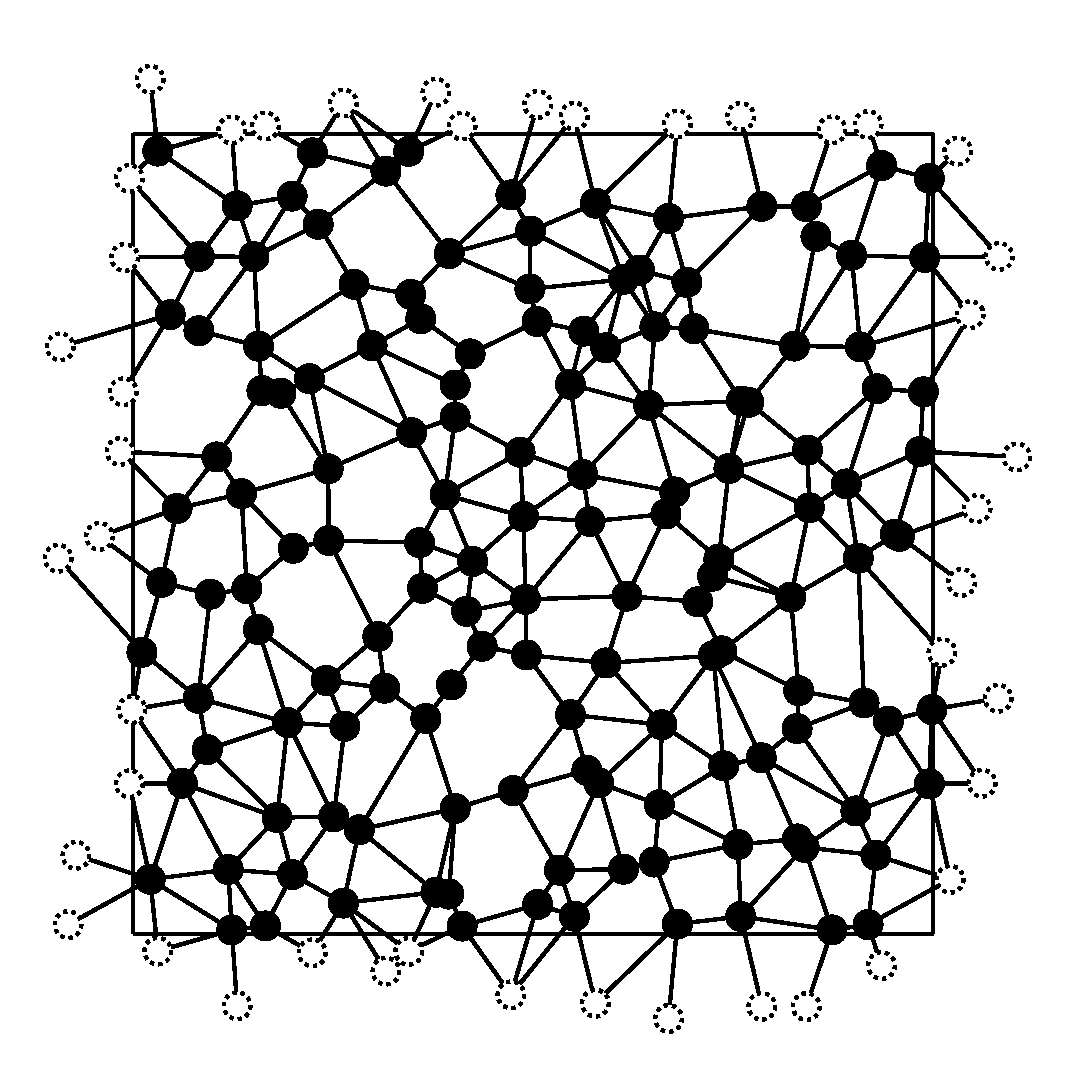
\includegraphics[width=0.3\textwidth]{images/GG/L12S03.pdf}
        }
        \caption[Gabriel - and Relative Neighborhood Graph]
        {
            \subref{sfig:lunes:def} Lunes of RNG (hatched region) and
                GG (cross hatched region)
            \subref{sfig:lunes:rng} Example of a RNG on periodic
                boundary conditions. Periodic nodes are dashed.
            \subref{sfig:lunes:gg} Example of a GG on
                periodic boundary conditions. Periodic nodes are dashed.
        }
        \label{fig:lunes}
    \end{figure}\\
    To construct these graphs the simple way is to test for each
    pair of nodes if any other node lies in
    the lune of the pair. That is of complexity \(O (N^3)\), because
    there are \(N(N-1)\) pairs and for each \(N-2\) nodes to test. So
    the product is of order \(O(N^3)\)\\
    To reduce the complexity one can first create a Delaunay
    Triangulation in complexity \(O (N \log N)\)
    \cite{RNGCell} and test the criterion for each edge, because
    the Delaunay triangulation is a supergraph of both. But the
    implementation of a Delaunay triangulation algorithm is not trivial
    and the generation of the graphs is not time critical in the scope
    of this bachelor thesis.\\
    So a trade off is to use basically the simple method but only test
    the criterion for nodes which are near to the lune and abort if
    one node inside the lune is found. To determine which nodes are
    near the lune one can subdivide the area in \emph{cells} and save
    for each cell a list with nodes lying inside it like presented in
    \cite{RNGCell}.
    Now it is just necessary to test the nodes in the cells which
    resemble a rectangular bounding box of the lune. Most pairs will be
    far away from each other and the cells in the middle of the bounding
    box are completely inside the lune so that only one node has to be
    tested to discard an edge between them. Connected nodes are near to
    each other so that only very few cells have to be tested.\\
    Indeed this method reduced the time needed to construct a RNG with
    \(N=32^2\) and \(N=64^2\) by a factor of
    over \(15\) respectively \(40\). Though the complexity is still of
    order \(O(N^2)\) in the best case, because for every pair at least
    one check has to be performed.
